\section{Future Work}


\subsection{Improve Robustness}
In this paper we have made many simplifications to the problem space just to make the placer easier to implement.
For example, our placer in its current state does not take advantage of \texttt{SLICEL}/\texttt{SLICEM} heterogeneity and simply maps all SLICE \texttt{SiteInst}s onto \texttt{SLICEL}s. 
Recall that the SLICE Sites in Xilinx FPGAs typically come in a 75-25\% split between \texttt{SLICEL}s and \texttt{SLICEM}s. 
This means that we have rendered about 25\% of the CLB fabric unusable which will inevitably hurt wirelength minimization during placement since the \texttt{SiteInst}s must be spread over a larger area. 
Enabling \texttt{SLICEL}-\texttt{SLICEM} heterogeneity can lead do greater logic density and consequently less total HPWL, but can make the packing process more complex and may contribute to higher routing congestion.

We can also add packing support for other Xilinx primitives such as the shift-register primitive \texttt{SRLx}, distributed RAM primitives \texttt{RAMSx}, or even \texttt{LATCH} primitives as discussed in \ref{sec:7_series}.
Adding support for additional primitives and macros will allow our placer to handle a wider range of HDL designs and will require deeper consideration of hardware constraints to ensure robustness.

In its current state, the prepacker and packer struggle to handle signals larger than 24-bits, especially when involved in DSP functions like addition and multiplication. 
In such designs, the Vivado synthesizer may synthesize long \texttt{CARRY4} chains with particular \texttt{EDIFHierPortInst} configurations which are currently not handled by our packer and lead to failures in the subsequent routing stage.
Further work is required to resolve these constraints in the packer.

\subsection{Force-Directed and Analytical Placement}
As discussed earlier, simulated annealing (SA) has largely been phased out in state-of-the-art (SOTA) placers due to its poor scalability and long runtimes. 
Our current placer follows a straightforward \emph{prepack–pack–place} flow, with the final placement stage driven by SA. 
In future work, this stage can be retrofitted to use analytical placement (AP) while reusing the prepacker and packer. 
Here, \texttt{SiteInst}s remain the atomic placement objects, and analytical solvers can be applied to minimize the total half-perimeter wirelength (HPWL) of the connecting nets.

The following works provide a foundation for understanding AP, ranging from early formulations to modern SOTA methods:
\begin{itemize}
    \item \emph{Analytical minimization of half-perimeter wirelength} — \textbf{Kennings and Markov (2000)} \cite{AP_2000}.
    \item \emph{Analytical placement for heterogeneous FPGAs} — \textbf{Gort et al. (2012)} \cite{AP_2012}.
    \item \emph{SimPL: An algorithm for placing VLSI circuits} — \textbf{Kim et al. (2013)} \cite{SimPL}.
    \item \emph{Multi-Electrostatic FPGA Placement Considering SLICEL–SLICEM Heterogeneity, Clock Feasibility, and Timing Optimization} — \textbf{Jing et al. (2023)} \cite{MultiElectrostatic}.
    \item \emph{OpenPARF 3.0: Robust Multi-Electrostatics Based FPGA Macro Placement Considering Cascaded Macro Groups and Fence Regions} — \textbf{Jing et al. (2024)} \cite{OpenPARF}.
\end{itemize}

As noted in Section~\ref{sec:placement}, replacing SA with AP requires splitting the placement stage into two substages:  
(1) \emph{global placement}, which determines continuous target positions using analytical optimization, and  
(2) \emph{detailed placement} (legalization), which snaps objects to valid \texttt{Site}s while adhering to hardware constraints.  
Global placement can be performed using any number of off-the-shelf (OTS) analytical solvers.

Unlike SA, which relies primarily on heuristics and probabilistic moves, AP begins with a formal mathematical formulation that is compatible with analytic optimization. 
As introduced in Section~\ref{subsec:netlist}, a circuit netlist can be naturally modeled as a \emph{hypergraph}
\[
    G_{H} = (V_{H}, E_{H}),
\]
where \(V_{H}\) is the set of vertices and \(E_{H}\) is the set of hyperedges, each of which may connect more than two vertices. 
In the FPGA context, \(V_{H}\) corresponds to the set of \texttt{SiteInst}s placed on the \texttt{device}, while \(E_{H}\) corresponds to the set of \texttt{Net}s interconnecting them.

We can then reduce this hypergraph into a graph by converting all multi-pin hyperedges into a set of 2-pin edges.

Most AP approaches then minimize the weighted sum of half perimeter wirelengths (HPWL) of these 2-pin edges, with some approaches using the sum of linear distances \ref{equ:Manhattan} and others using the sum of squared distances \ref{equ:Euclidian}.


\begin{equation}
    \boldsymbol{\Phi} (\vec{x}, \vec{y}) = \sum_{i,j} w_{i,j} \left( |x_i - x_j| + |y_i - y_j| \right)
    \label{equ:Manhattan}
\end{equation}

\begin{equation}
    \boldsymbol{\Phi} (\vec{x}, \vec{y}) = \sum_{i,j} w_{i,j} \left[ (x_i - x_j)^2 + (y_i - y_j)^2 \right]
    \label{equ:Euclidian}
\end{equation}

% use these formulations
% HPWL_AP_2000
% HPWL_AP_2012






\subsection{Variations on Packing}
Our current placer follows a \textbf{Site-centric} approach that resembles that of the old Xilinx ISE - the predecessor to Vivado used in the 90s and 2000s.
These days, Vivado performs \textbf{BEL-centric} placement without necessarily locking \texttt{Cell}s into \texttt{Site}s, allowing for a higher granularity of movement of \texttt{Cell}s. 
Enabling BEL-centric moveme
nt as opposed to Site-centric movement can improve HPWL minimization, but will add much more complexity to the packing and placement process to ensure robustness with respect to hardware constraints.

There is no constraint that forces us to pack \texttt{Cells} into \texttt{SiteInst}s before placement or to follow a strict prepacking-packing-placement flow. 
After implementing a force-directed or analytical placer, we can begin to explore different packing and placement ordering like those studied in Wuxi et al. (2019) \cite{ExplicitPacking}.

{
    \centering
    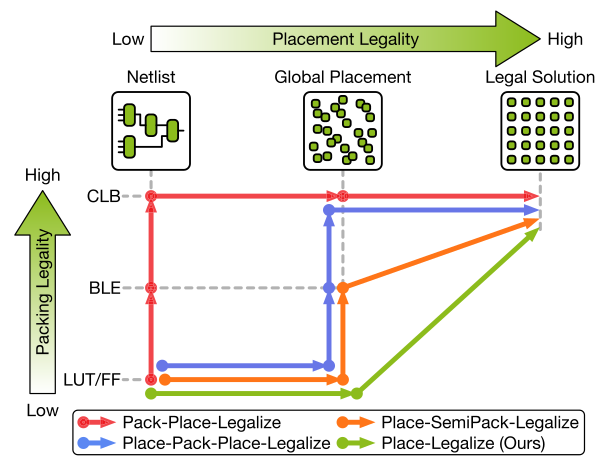
\includegraphics[width=\columnwidth]{figures/future_work/legalization.png}
    \captionof{figure}{Representative FPGA placement and packing flows. Figure taken from Wuxi et al. (2019), page 1 \cite{ExplicitPacking}}
}
\vspace{0.25cm}

\subsection{Add Hard Macro Support}






